\section{Auswertung}
\subsection{Untersuchung des Linearverstärkers}
Die Untersuchung der verschiedenen Linearverstärker beginnt mit der Bestimmung der Grenzfrequenz $v'_g$. Hierzu wird die Ausgangsspannung gegen die Frequenz aufgetragen und danach die Anhängigkeit der Verstärkung von der Frequenz untersucht. Die Grenzfrequenz ist dann diejenige, bei welcher die Verstärkung $V'$ auf $\frac{V'}{\sqrt{2}}$ abgefallen ist.
Die Widerstandswerte für die Linearverstärker sind in Tabelle \ref{Tab_2} zu finden. Der Ausgangsspannungsverlauf des ersten Verstärkers ist in Abb.\ref{plot1} dargestellt.
\begin{figure}[h]
  \centering
  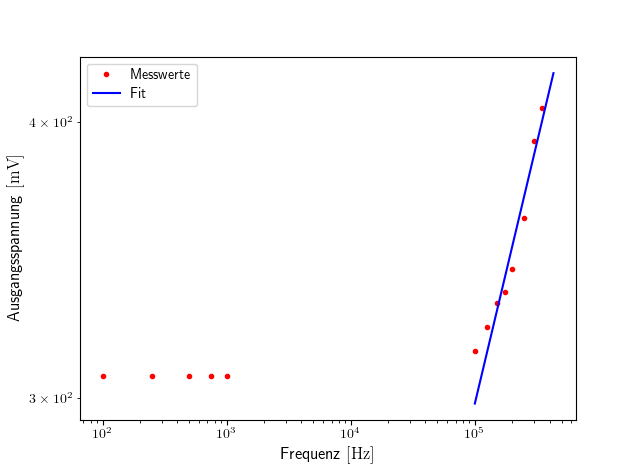
\includegraphics[width=1\textwidth]{bilder/Figure_1.png}
  \caption{Frequenzverlauf der Ausgangsspannung mit Fit an der steigenden Seite.}
  \label{Aufbau}
\end{figure}
Hierbei wird neben dem Darstellen der Messwerte noch ein Fit der Form
\begin{equation}
f(x)=mx^b
\end{equation}
durchgeführt um die Steigung der Gerade im doppeltlogarithmischen Plot zu bestimmen. Die Ergebnisse der Fits für die unterschiedlichen Linearverstärker sind in Tabelle \ref{Tab_1} eingetragen.
\begin{table}[]
\centering
\begin{tabular}{c|ccc}
&$R_1\,[\si{\kilo\ohm}]$&$R_2\,[\si{\kilo\ohm}]$&Verstärkungsfaktor\\
\hline
Verstärker 1 & 100 & 10  &$1/10$\\
Verstärker 2 & 100 & 1   &$1/100$\\
Verstärker 3 & 10  & 0,5 &$1/20$\\
Verstärker 4 & 10  & 33  &$3{,}3$
\end{tabular}
\label{Tab_2}
\end{table}
\begin{figure}[h]
  \centering
  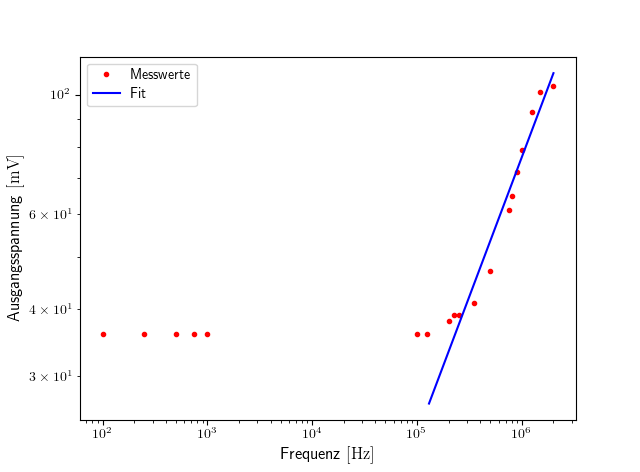
\includegraphics[width=1\textwidth]{bilder/Figure_2.png}
  \caption{Frequenzverlauf der Ausgangsspannung des zweiten Linearverstärkers mit Fit an der steigenden Seite.}
  \label{Aufbau}
\end{figure}
\begin{figure}[h]
  \centering
  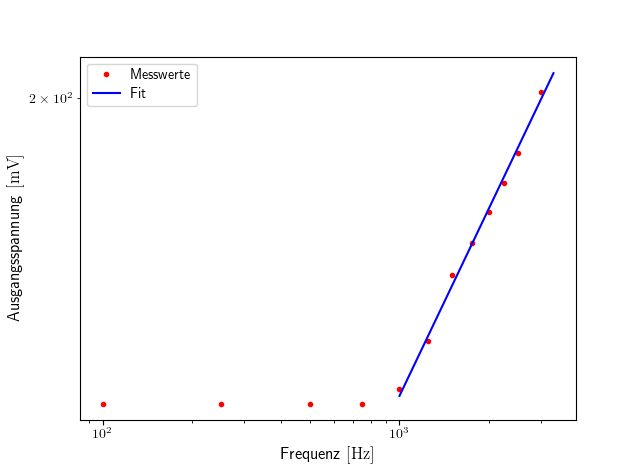
\includegraphics[width=1\textwidth]{bilder/Figure_3.png}
  \caption{Darstellung des Frequenzverlaufs der Ausgangsspannung am dritten Linearverstärker mit Fit an der steigenden Seite.}
  \label{Aufbau}
\end{figure}
\begin{figure}[h]
  \centering
  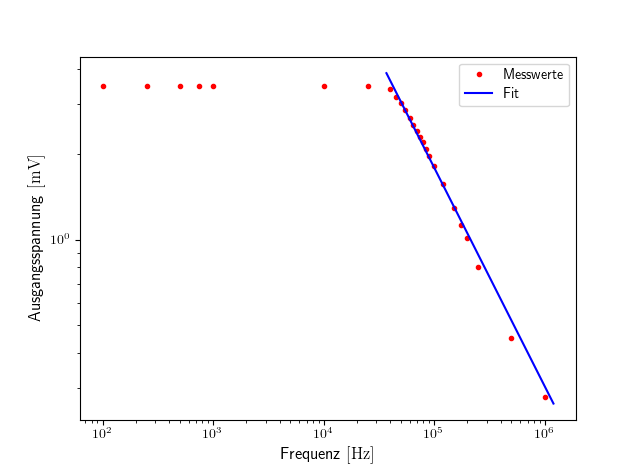
\includegraphics[width=1\textwidth]{bilder/Figure_4.png}
  \caption{Frequenzabhängigkeit der Ausgangsspannung des vierten Linearverstärkers mit Fit an der fallenden Seite.}
  \label{Aufbau}
\end{figure}
Es lässt sich nun die Grenzfrequenz für die einzelnen Linearverstärker bestimmen indem die Fitfunktion invertiert wird und der Frequenzwert für $U_A=\frac{U'_\text{const}}{\sqrt{2}}$, wobei $U'_\text{const}$ die Spannung am konstanten Teil der Kurve ist, berechnet wird:
\begin{equation}
  \nu_g=\left(\frac{U'_\text{const}}{\sqrt{2}m}\right)^{\frac{1}{b}}
\end{equation}
Es ergibt sich für die verschiedenen Linearverstärker
\begin{table}[H]
\centering
\begin{tabular}{c|cc}
&$m\,[\frac{\si{\mV}}{\si{\kHz}}]$&$b$\\
\hline
Verstärker 1 & $24\pm 9$ & $0{,}218\pm 0{,}031$\\
Verstärker 2 & $0{,}61\pm0{,}3$ & $0{,}52\pm0{,}04$   \\
Verstärker 3 & $27{,}4\pm2{,}0$ & $0{,}248\pm0{,}009$   \\
Verstärker 4 & $(1{,}26\pm0{,}24)\cdot10^4$ & $-0{,}769\pm0{,}017$   \\
\end{tabular}
\label{Tab_3}
\end{table}
%%%%%%%%%%%%%%%%%%%%%%%%%%%%%%%%%%%%%%%%%%%%%%%%%%
\subsection{Untersuchung des Umkehr-Integrators und Differentiators}
Es wird untersucht in welchem Bereich die theoretischen Zusammenhänge zwischen Ausgangsspannung und Frequenz erfüllt sind. Hierzu wird erneut die Ausgangsspannung für beide Aufbauten doppeltlogarithmisch gegen die Frequenz aufgetragen und die Steigung der auftretenden Gerade durch einen Fit ermittelt. Die Messwerte sowie die Ausgleichskurven sind in den Abb.\ref{integrator} und Abb.\ref{differentiator} dargestellt. Für beide Schaltungen wurde ein Kondensator mit einer Kapazität von $F=0{,}015\,\si{\micro\farad}$ und ein Widerstand mit $R=10\,\si{\kilo\ohm}$ genutzt. Für die Fitfunktion der Form:
\begin{equation}
U_A=m\cdot\nu^b\,,
\end{equation}
ergeben sich die Parameter:
\begin{align}
\text{Umkehr-Differentiator:}&\quad \left(0{,}53\pm0{,}08\right)\frac{1}{\si{\Hz}}\cdot\nu^{1{,}01\pm0{,}03} \nonumber\\
\text{Umkehr-Integrator:}&\quad \left(177\pm10\right)\frac{1}{\si{\Hz}}\cdot\nu^{-0{,}814\pm0{,}02}\nonumber
\end{align}
Für den Umkehr-Differentiator ist festzustellen, dass der erwartete Zusammenhang zwischen Ausgangsspannung und Frequenz nur zwischen ca. $100\,\si{\Hz}\.-\.800\,\si{\Hz}$ vorliegt. Beim Umkehr-Integrator hingegen findet sich kein Bereich in welchem der theoretische Verlauf nicht erfüllt wird. Die integrierenden und differentierenden Eigenschaften der Schaltungen sind in den folgenden Oszilloskopbildern gut zu erkennen, hierbei ist das Eingangssignal stets gelb un das Signal der Schaltung grün.
\begin{figure}[h]
  \centering
  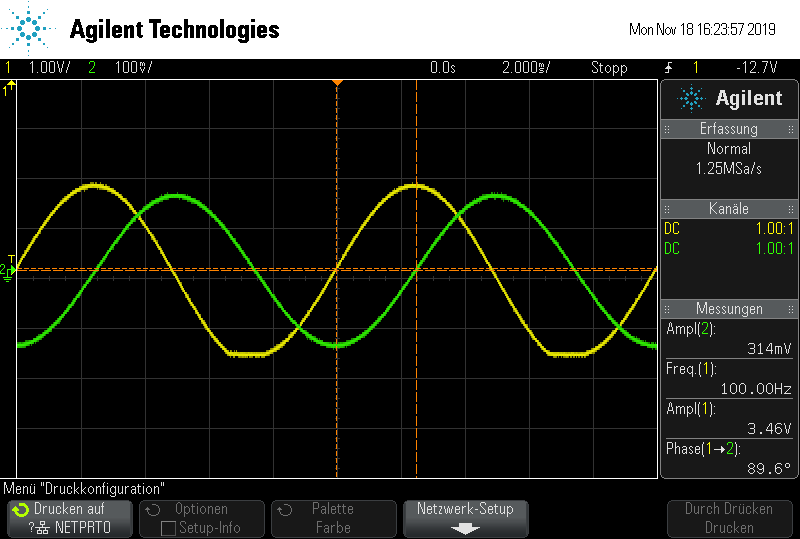
\includegraphics[width=1\textwidth]{bilder/integrator1.png}
  \caption{Integrierte Sinusspannung}
\end{figure}
\begin{figure}[h]
  \centering
  \includegraphics[width=1\textwidth]{bilder/integrator2.png}
  \caption{Integrierte Dreiecksspannung}
\end{figure}
\begin{figure}[h]
  \centering
  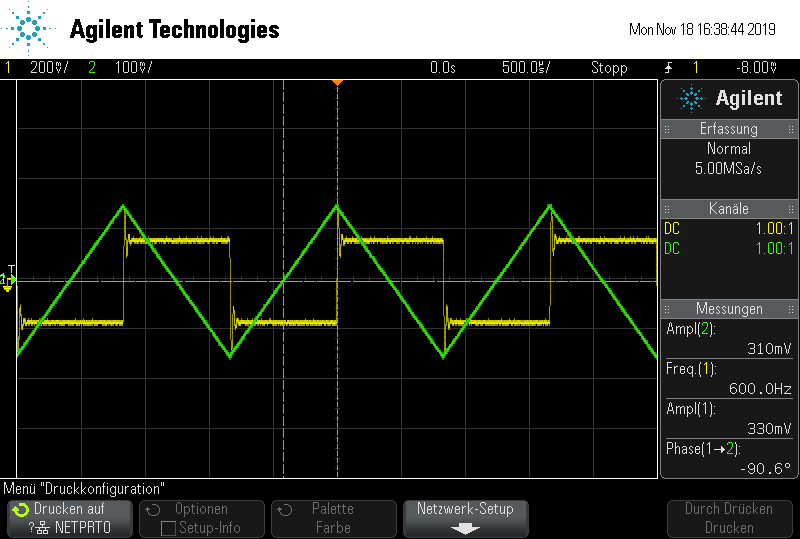
\includegraphics[width=1\textwidth]{bilder/integrator3.png}
  \caption{Integrierte Rechtecksspannung}
\end{figure}
\begin{figure}[h]
  \centering
  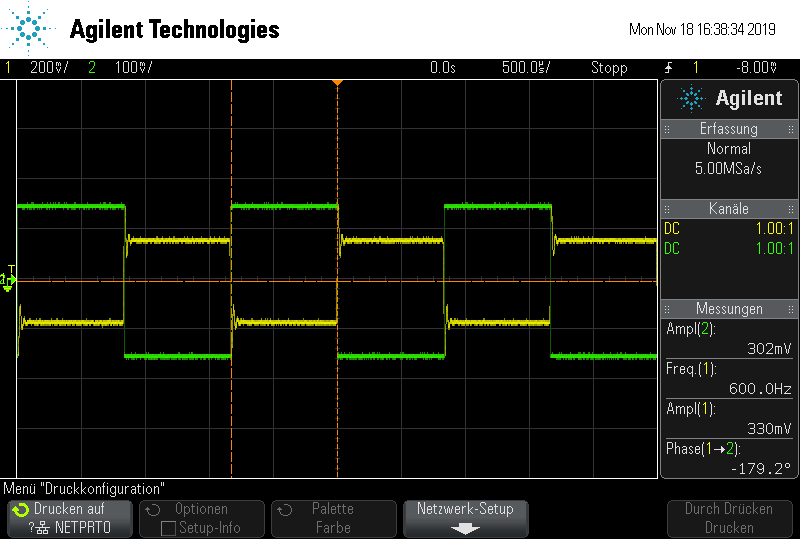
\includegraphics[width=1\textwidth]{bilder/diff1.png}
  \caption{Differentierte Rechtecksspannung}
\end{figure}
\begin{figure}[h]
  \centering
  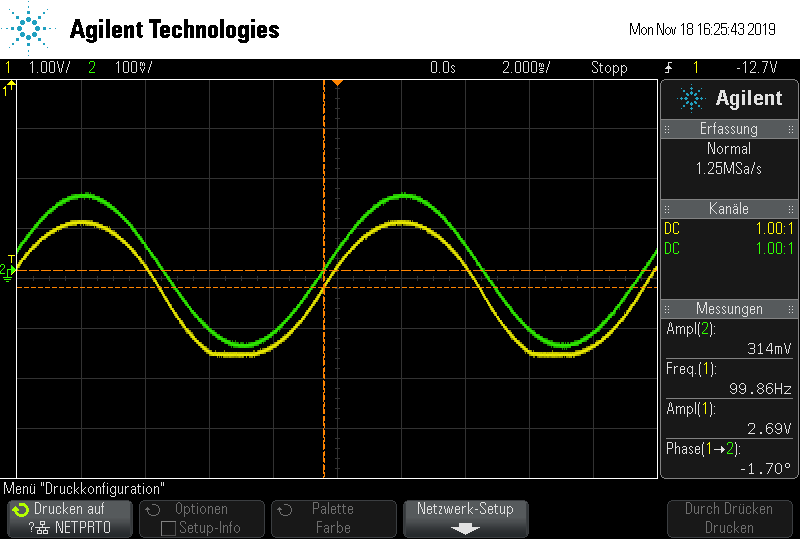
\includegraphics[width=1\textwidth]{bilder/diff2.png}
  \caption{Differentierte Sinusspannung?}%Vllt auch rausnehmen
\end{figure}
\subsection{Der Schmitt-Trigger}
Die technischen Daten des Aufbaus des Schmitt-Triggers sind:
\begin{table}[]
\centering
\begin{tabular}{ccc}
$U_{B,+}=12{,}75 \,\si{\V}$ \\
$U_{B,-}=-13{,}8\,\si{V}$ \\
$R_1=10\,\si{\kilo\ohm}$ \\
$R_p=33\,\si{\kilo\ohm}$ \\
\end{tabular}
\end{table}
Mit (15) ergibt sich dann ein theoretischer Umschlagpunkt von
\begin{equation}
U_{+,\text{theo}}=3{,}86\,\si{\V}
\end{equation}
Der gemessene Schwellwert liegt bei
\begin{equation}
U_{+}=4{,}15\,\si{\V}
\end{equation}
